\chapter{Statique du Solide}
\begin{itemize}
	\item[Statique :] étude des solides en \ul{equilibre} sous l'action \ul{de forces}.
	\item[force :] action exercée sur un solide / un point matériel. Elle est définie par son intensité, sa direction, son sens. La force est toujours prise comme une quantité vectorielle.
		Un vecteur se note par $\vec{AB}$
	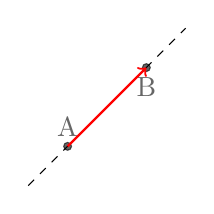
\begin{tikzpicture}
		\draw[dashed] (0, 0) -- (2, 2);
		\draw[fill=black, opacity=0.6] (0.5, 0.5) circle (0.05) node [above] {A};
		\draw[fill=black, opacity = 0.6] (1.5, 1.5) circle (0.05) node [below] {B};
		\draw[->, red, thick] (0.5, 0.5) -- (1.5, 1.5);
	\end{tikzpicture}
\end{itemize}

\section{Quelques forces}
\paragraph{La force de gravitation}
\begin{wrapfigure}{r}{0pt}
	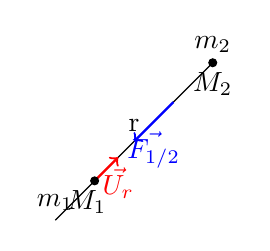
\begin{tikzpicture}
		\draw (0, 0) -- (2, 2) node [above, midway] {r};
		\draw[->, red, thick] (0.5, 0.5) -- (0.8, 0.8) node [below] {$\vec{U_r}$};
		\draw[->, blue, thick] (1.5, 1.5) -- (1, 1) node [midway, below] {$\vec{F_{1/2}}$};
		\draw[fill=black] (0.5, 0.5) circle (0.05) node [xshift=-0.1cm, below] {$M_1$};
		\draw[fill=black] (2, 2) circle (0.05) node [below] {$M_2$};
		\node at (2,2) [above] {$m_2$};
		\node at (0,0) [above] {$m_1$};
	\end{tikzpicture}
\end{wrapfigure}
	C'est une force attractive, elle est exercée par une masse $M_1$ en présence d'une autre masse $M_2$
\begin{align*}
	\overrightarrow{F_{1/2}} &=& - \frac{G*m_1*m_2}{||\overrightarrow{M_1M_2}||^2}*\frac{\overrightarrow{M_1M_2}}{||\overrightarrow{M_1M_2}||} \\
	&=& -\frac{G*m_1*m_2}{r^2}\overrightarrow{u_r}
\end{align*}

\begin{itemize}
	\item[G :] Constante de gravitation $G=6.67*10^{-11} m^3kg^{-1}s^{-2}$
	\item[$m_1, m_2$ :] Masses des corps 1 et 2
	\item[$M_1, M_2$ :] Position des corps 1 et 2
\end{itemize}

\paragraph{Remarques}

\begin{itemize}
	\item[] Force gravitationnelle inversemment proportionelle à $r^2$. Sa portée est donc infinie
	\item[] Elle fait partie des forces fondamentales.
	\item[] Elle est cependant mal connu aux petites échelles (subatomique).
\end{itemize}
C'est la force de gravitation qui régule la distribution des structures dans la nature.

\paragraph{La force électrostatique}
\begin{wrapfigure}{r}{0pt}
	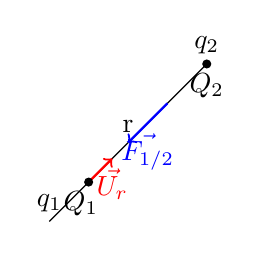
\begin{tikzpicture}
		\draw (0, 0) -- (2, 2) node [above, midway] {r};
		\draw[->, red, thick] (0.5, 0.5) -- (0.8, 0.8) node [below] {$\vec{U_r}$};
		\draw[->, blue, thick] (1.5, 1.5) -- (1, 1) node [midway, below] {$\vec{F_{1/2}}$};
		\draw[fill=black] (0.5, 0.5) circle (0.05) node [xshift=-0.1cm, below] {$Q_1$};
		\draw[fill=black] (2, 2) circle (0.05) node [below] {$Q_2$};
		\node at (2,2) [above] {$q_2$};
		\node at (0,0) [above] {$q_1$};
	\end{tikzpicture}
\end{wrapfigure}
Elle s'exerce entre 2 charges à \ul{l'immobiles}.
\begin{align*}
	\overrightarrow{F} &=& -\frac{1}{4*\pi*\epsilon_0}*{Q_1Q_2}\frac{1}{r^2}\vec{u_r} \text{ Force de coulomb}\\
	\epsilon_0 &=& 8.854*10^{-2} F.m ^{-2} 
\end{align*}
\begin{itemize}
	\item[$\epsilon_0$ : ] Permittivité du \ul{vide}
\end{itemize}

\paragraph{Remarque} Elle est similaire dans la forme à la force de gravitation mais
$
	\left. 
	\begin{array}{r c l}
		Q &=& > 0 \\
		Q &=& < 0
	\end{array}
	\right\}
$
Elle est la principal cause de la cohésion de la matière : La cohésion dans un atome (entre les charge $e^-$ et $e^+$) et celle des molécules.
\begin{align*}
	[Q]&=&I.T\\
	\text{Unité(Q)}&=& \text{Coulomb (C)}
\end{align*}

\paragraph{Force de frottement fluide/visqueux}
Force exercée par un fluide sur un solide en \ul{mouvement} par rapport au fluide.
\begin{align*}
	F&=&-f.\vec{v}\\
	f&=& \text{coefficient nummérique de frottement dépend de la nature du fluide.}
\end{align*}
l'origine de cette force est l'interaction moléculaire des fluides et solides.
\paragraph{Remarque} La forme est valable uniquement si v n'est pas trop grand.

\paragraph{force de frottement solide}
\begin{wrapfigure}{r}{0pt}
	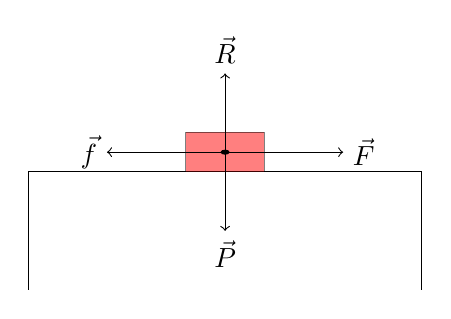
\begin{tikzpicture}[yscale=0.5]
	\draw[] (0, -3)  -- (0, 0) -- (5, 0) -- (5, -3);
	\draw[fill=red, opacity=0.5] (2, 1) rectangle (3, 0);
	\draw[<->] (1, 0.5) -- (4, 0.5) node [right] {$\vec{F}$};
	\node at (1, 0.5) [left] {$\vec{f}$};
	\draw[<->] (2.5, -1.5) -- (2.5, 2.5) node [above] {$\vec{R}$};
	\node at (2.5, -1.5) [below] {$\vec{P}$};
	\draw[fill=black] (2.5, 0.5) circle (0.05);
\end{tikzpicture}
\end{wrapfigure}
~\\
Si $||\vec{F}|| > ||\vec{P}||.k_s$ \\ Alors le corps est en mouvement. $k_s=$coefficient de frottement statique \\
$\vec{F} = $ Force exercé sur le corps.

Le support exerce une force \[
	\left.
	\begin{array}{l}
		\text{Si } ||\overrightarrow{f_s}|| < k_smg\\
	\text{Le solide reste statique : la force de frottement opposé} \\
	\text{aux mouvement est appelé force de frottement du solide \ul{statique}}\\
	\text{F est la force de frottement statique du solide}
	\end{array}
	\right\}
\]

Quand $\vec{F}$ devient suffisante ($||\overrightarrow{f_c} = k_c*mg||$), le solide est en mouvement. La force de frottement opposé à la force de déplacement est appelé force de frottement du solide \ul{cinetique}.

$k_c < k_s$ avec $k_c$ le coefficient de frottement cinématique et $k_s$ le coefficient de frottement statique, et on a $||\overrightarrow{f_c}|| < ||\overrightarrow{f_s}||$
\paragraph{Remarque} Les forces de frottements statique et cinétique ne dépende que le nature des 2 surfaces en contacte. Elle ne dépend pas par exemple de la vitesse.
Elle est du aux interactions entre les atomes et les molécules en surfaces.


\paragraph{Force élastique (ou de rappel)} C'est la force qu'exerce un solide pour s'opposer à une déformation.

\begin{wrapfigure}{r}{0pt}
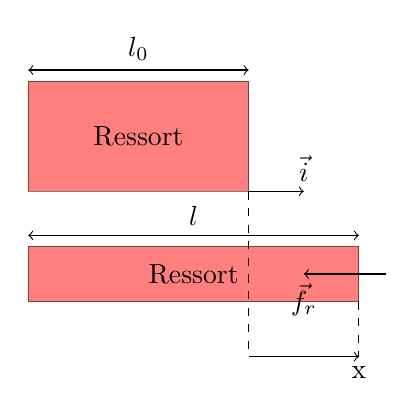
\begin{tikzpicture}[scale=0.7]
	\draw[fill=red, opacity=0.5] (0, 2) rectangle (4, 0);
	\node at (2, 1) {Ressort};
	\draw[<->] (0, 2.2) -- (4, 2.2) node [midway, above] {$l_0$};
	\draw[fill=red, opacity=0.5] (0, -1) rectangle (6, -2);
	\draw[<->] (0, -0.8) -- (6, -0.8) node [midway, above] {$l$};
	\draw[->] (6.5, -1.5) -- (5, -1.5) node [below] {$\vec{f_r}$};
	\draw[->] (4, 0) -- (5, 0) node [above] {$\vec{i}$};
	\draw[->] (4, -3) -- (6, -3) node [below] {x};
	\node at (3, -1.5) {Ressort};
	\draw[dashed] (4, 0) -- (4, -3);
	\draw[dashed] (6, -2) -- (6, -3);
\end{tikzpicture}
\end{wrapfigure}
$l_0$ est la longueur au repos du ressort et l la longueur du ressort après deformation
\begin{align*}
	\overrightarrow{F_r} &=& -k(l-l_0)*\vec{i} \\
										&=& -k.x.\vec{i}, \text{ avec }x=(l-l_0)
\end{align*}
k est la constante de raideur du ressort, la forme $\vec{F_r} = -k.x.\vec{i}$ n'est valable que si on comprime le ressort ($x<0$).

Si on déforme trop le solide (si on quitte le domaine élastique), d'après la loi de Hook, le solide entre dans le domaine plastique et ne revient plus à sa longueur original.
